% \documentclass[aspectratio=169,notes]{beamer}
\documentclass[aspectratio=169]{beamer}
\usetheme[faculty=phil]{fibeamer}
\usepackage{polyglossia}
\setmainlanguage{english} %% main locale instead of `english`, you
%% can typeset the presentation in either Czech or Slovak,
%% respectively.
\setotherlanguages{russian} %% The additional keys allow
%%
%%   \begin{otherlanguage}{czech}   ... \end{otherlanguage}
%%   \begin{otherlanguage}{slovak}  ... \end{otherlanguage}
%%
%% These macros specify information about the presentation
\title[IME]{Introduction to Mechanical Engineering, Lecture 7} %% that will be typeset on the
\subtitle{Engineering Materials:  
\\ Steel, Bronze, Aluminium, Titanium, Composites  \\   
\ } %% title page.
\author{Oleg Bulichev}
%% These additional packages are used within the document:
\usepackage{ragged2e}  % `\justifying` text
\usepackage{booktabs}  % Tables
\usepackage{tabularx}
\usepackage{tikz}      % Diagrams
\usetikzlibrary{calc, shapes, backgrounds}
\usetikzlibrary{decorations.pathreplacing,calligraphy,calc,graphs}
\usepackage{amsmath, amssymb}
\usepackage{url}       % `\url`s
\usepackage{listings}  % Code listings
% \usepackage{subfigure}
\usepackage{floatrow}
\usepackage{subcaption}
\usepackage{mathtools}
\usepackage{todonotes}
\usepackage{fontspec}
\usepackage{multicol}
\usepackage{pdfpages}
\usepackage{wrapfig}
\usepackage{animate}
\usepackage{booktabs}
\usepackage{multirow}
% \usepackage{graphicx}
\usepackage{colortbl}

\graphicspath{{resources/}}
\frenchspacing

\setbeamertemplate{caption}[numbered]
\usetikzlibrary{graphs}

% \usepackage[backend=biber,style=ieee,autocite=footnote]{biblatex}
% \addbibresource{biblio.bib}
% \DefineBibliographyStrings{english}{%
%   bibliography = {References},}

\newcommand{\oleg}[2][] {\todo[color=red, #1] {OLEG:\\ #2}}
\newcommand{\fbckg}[1]{\usebackgroundtemplate{\includegraphics[width=\paperwidth]{#1}}}%frame background

\usepackage[framemethod=TikZ]{mdframed}
\newcommand{\dbox}[1]{
\begin{mdframed}[roundcorner=3pt, backgroundcolor=yellow, linewidth=0]
\vspace{1mm}
{#1}
\vspace{1mm}
\end{mdframed}
}

\begin{document}
\setlength{\abovedisplayskip}{0pt}
\setlength{\belowdisplayskip}{0pt}
\setlength{\abovedisplayshortskip}{0pt}
\setlength{\belowdisplayshortskip}{0pt}

\fbckg{fibeamer/figs/title_page.png}
\frame[c]{\setcounter{framenumber}{0}
    \usebeamerfont{title}%
    \usebeamercolor[fg]{title}%
    \begin{minipage}[b][6.5\baselineskip][b]{\textwidth}%
        \textcolor{black}{\raggedright\inserttitle}
    \end{minipage}
    % \vskip-1.5\baselineskip

    \usebeamerfont{subtitle}%
    \usebeamercolor[fg]{framesubtitle}%
    \begin{minipage}[b][3\baselineskip][b]{\textwidth}
        \raggedright%
        \insertsubtitle%
    \end{minipage}
    \vskip.25\baselineskip
}
%   \frame[c]{\maketitle}

\fbckg{fibeamer/figs/common.png}

\note{\scriptsize \begin{itemize}
        \item \
    \end{itemize}}

    \begin{frame}[t]{Invited Lecturer Musa (RUS)}
        \framesubtitle{Video, Part 1}
        \vspace{-0.6cm}
        \begin{figure}[H]
            \href{https://disk.yandex.ru/i/pmZGYsEMQlrWTA}{
                \centering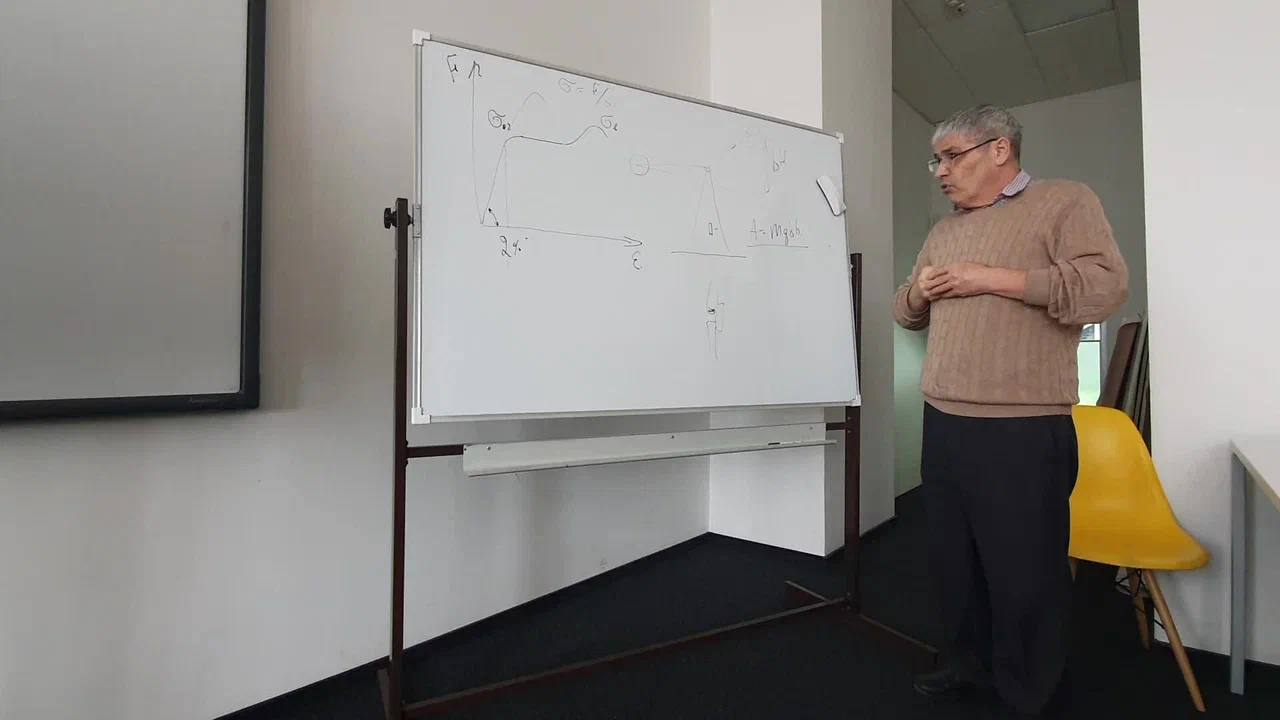
\includegraphics[height=6cm,width=1\textwidth,keepaspectratio]{musa_lec_1_video.png}}
            \label{fig:musa_lec_1_video.png}
        \end{figure}
    \end{frame}
    
    \begin{frame}[t]{Invited Lecturer Musa (RUS)}
        \framesubtitle{Video}
        \vspace{-0.6cm}
        \begin{figure}[H]
            \href{https://disk.yandex.ru/i/RtD8vtzjY-XxyQ}{
                \centering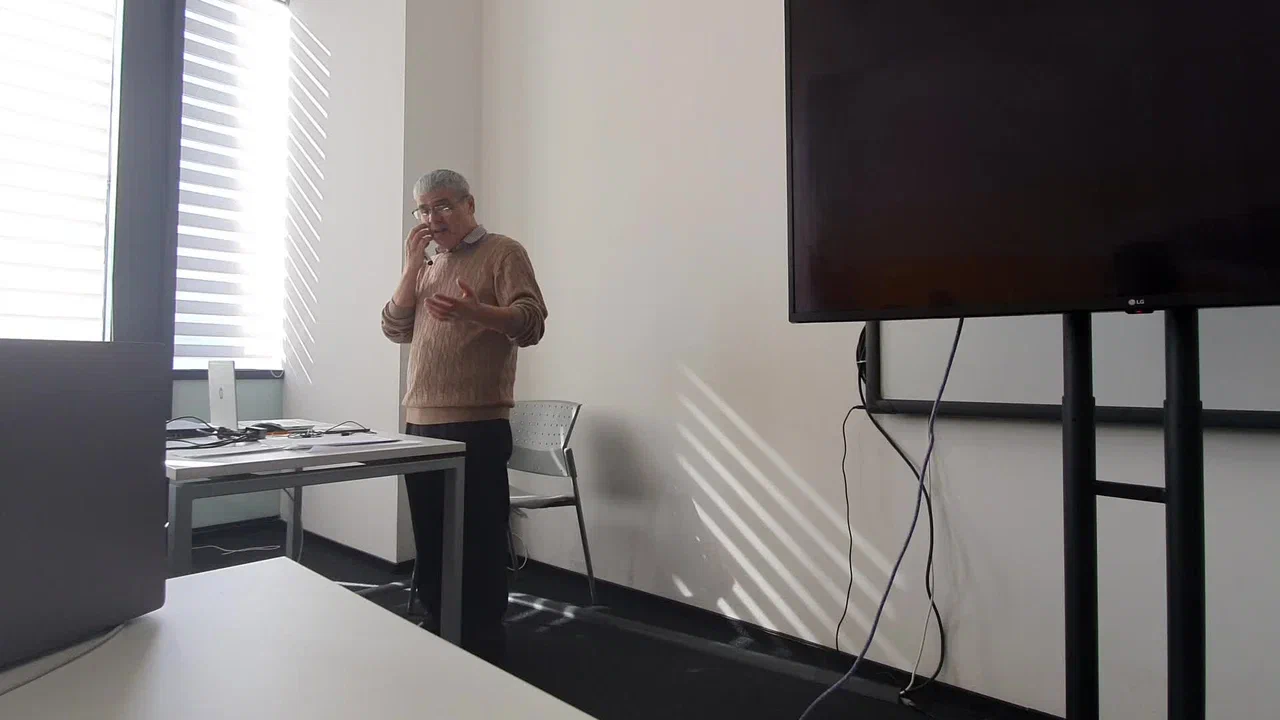
\includegraphics[height=6cm,width=1\textwidth,keepaspectratio]{musa_lec_2_video.png}}
            \label{fig:musa_lec_2_video.png}
        \end{figure}
    \end{frame}

\begin{frame}[t]{Understanding Metals (ENG)}
    \framesubtitle{Video}
    \vspace{-0.6cm}
    \begin{figure}[H]
        \href{https://youtu.be/PaGJwOPg2kU}{
            \centering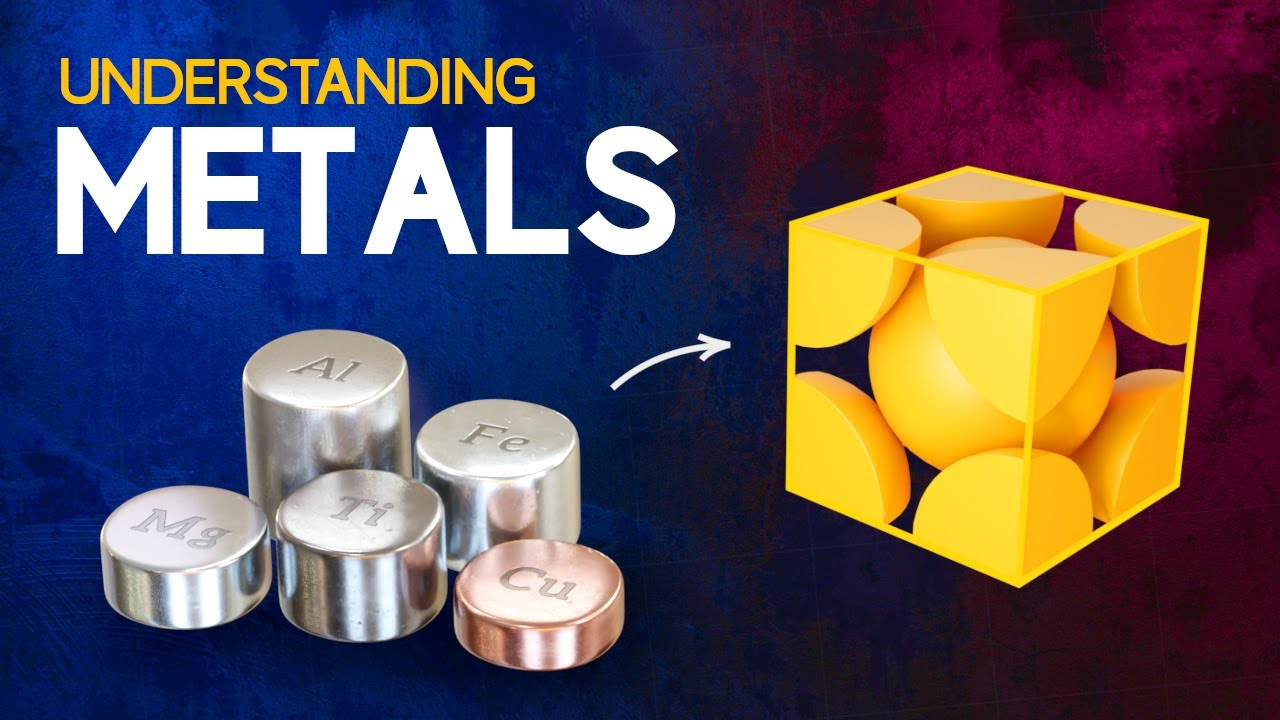
\includegraphics[height=6cm,width=1\textwidth,keepaspectratio]{understand_metals_video.jpg}}
        \label{fig:understand_metals_video.jpg}
    \end{figure}
\end{frame}

\begin{frame}[t]{Iron - Carbon plot (RUS)}
    \framesubtitle{}
        \vspace{-0.6cm}
        \begin{figure}[H]
            \centering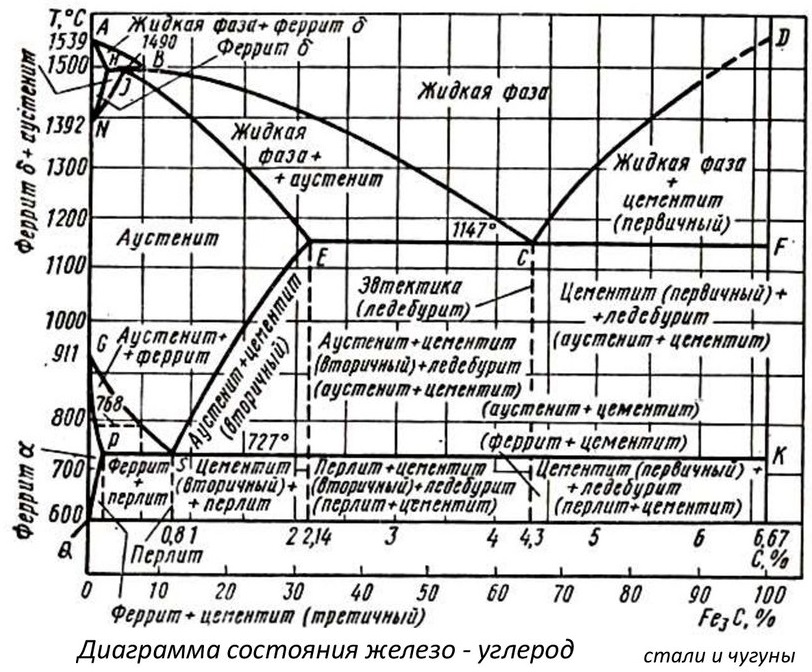
\includegraphics[height=6.4cm,width=1\textwidth,keepaspectratio]{FeCplot.jpg}
            \label{fig:FeCplot.jpg}
        \end{figure}
    \end{frame}

\begin{frame}[t]{Alloying Elements (Легирующие добавки)}
\framesubtitle{}
    \vspace{-0.6cm}
    \begin{figure}[H]
        \centering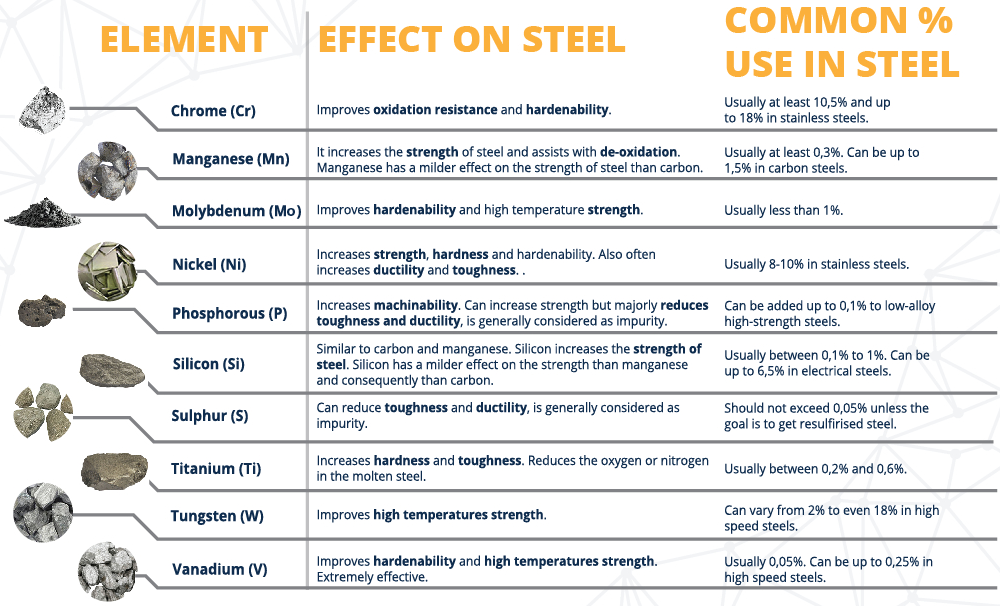
\includegraphics[height=6.4cm,width=1\textwidth,keepaspectratio]{alloy_elements.png}
        \label{fig:alloy_elements.png}
    \end{figure}
\end{frame}

\begin{frame}[t]{Alloying Elements (RUS)}
\framesubtitle{}
    \vspace{-0.6cm}
    \begin{figure}[H]
        \centering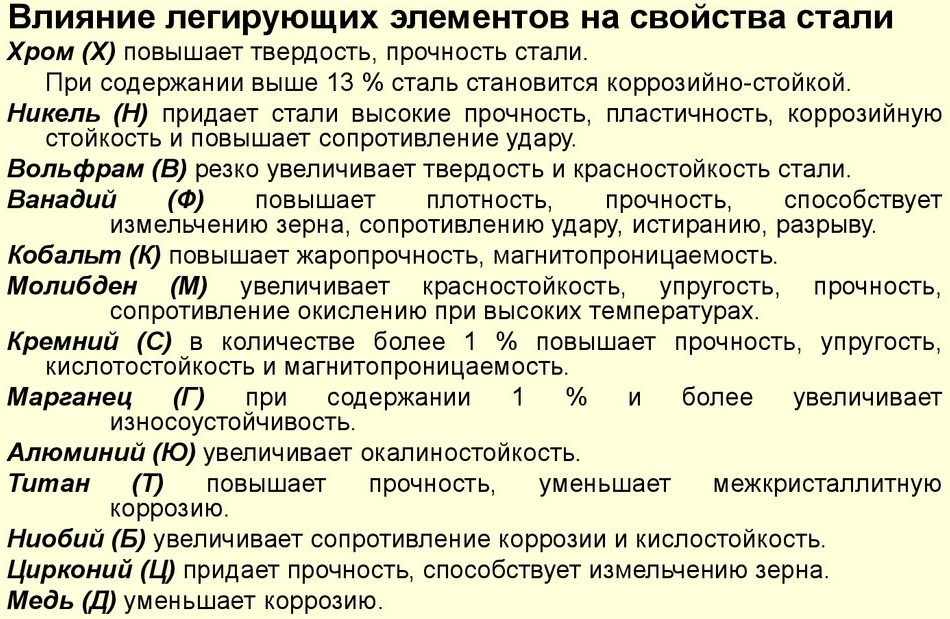
\includegraphics[height=6.4cm,width=1\textwidth,keepaspectratio]{fig2.jpeg}
        \label{fig:fig2.jpeg}
    \end{figure}
\end{frame}


\begin{frame}[t]{Understanding Durability of Metals (ENG)}
    \framesubtitle{Video}
    \vspace{-0.6cm}
    \begin{figure}[H]
        \href{https://youtu.be/WSRqJdT2COE}{
            \centering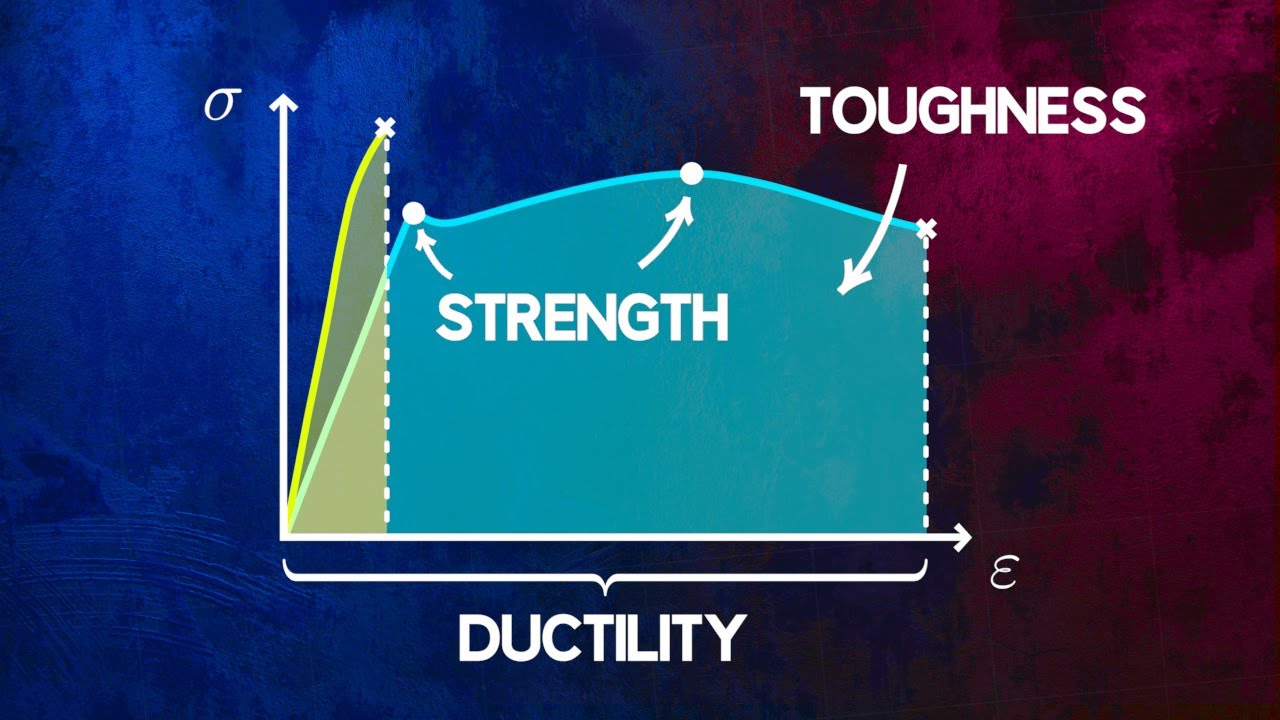
\includegraphics[height=6cm,width=1\textwidth,keepaspectratio]{understand_strength_video.jpg}}
        \label{fig:understand_strength_video.jpg}
    \end{figure}
\end{frame}

\begin{frame}[t]{Identifyning Steels (Расшифровка марок сталей)}
\framesubtitle{}
    \vspace{-0.6cm}
    \begin{figure}[H]
        \centering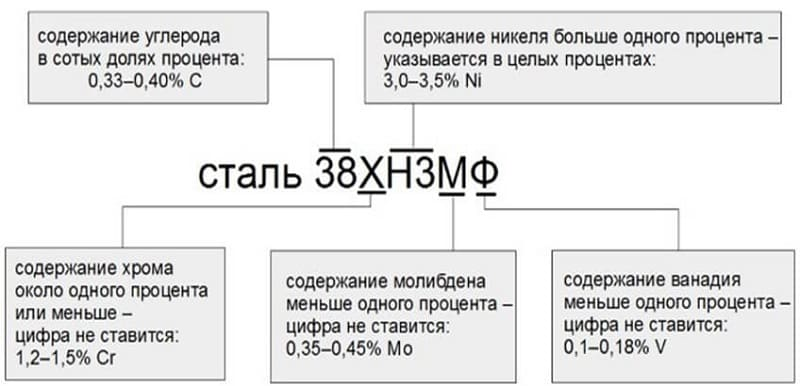
\includegraphics[height=6cm,width=1\textwidth,keepaspectratio]{rus_marker.jpg}
        \label{fig:rus_marker.jpg}
    \end{figure}
\end{frame}

\begin{frame}[t]{Identifyning Steels (ENG)}
    \framesubtitle{Video}
    \vspace{-0.6cm}
    \begin{figure}[H]
        \href{https://youtu.be/gXXRGjddQOM}{
            \centering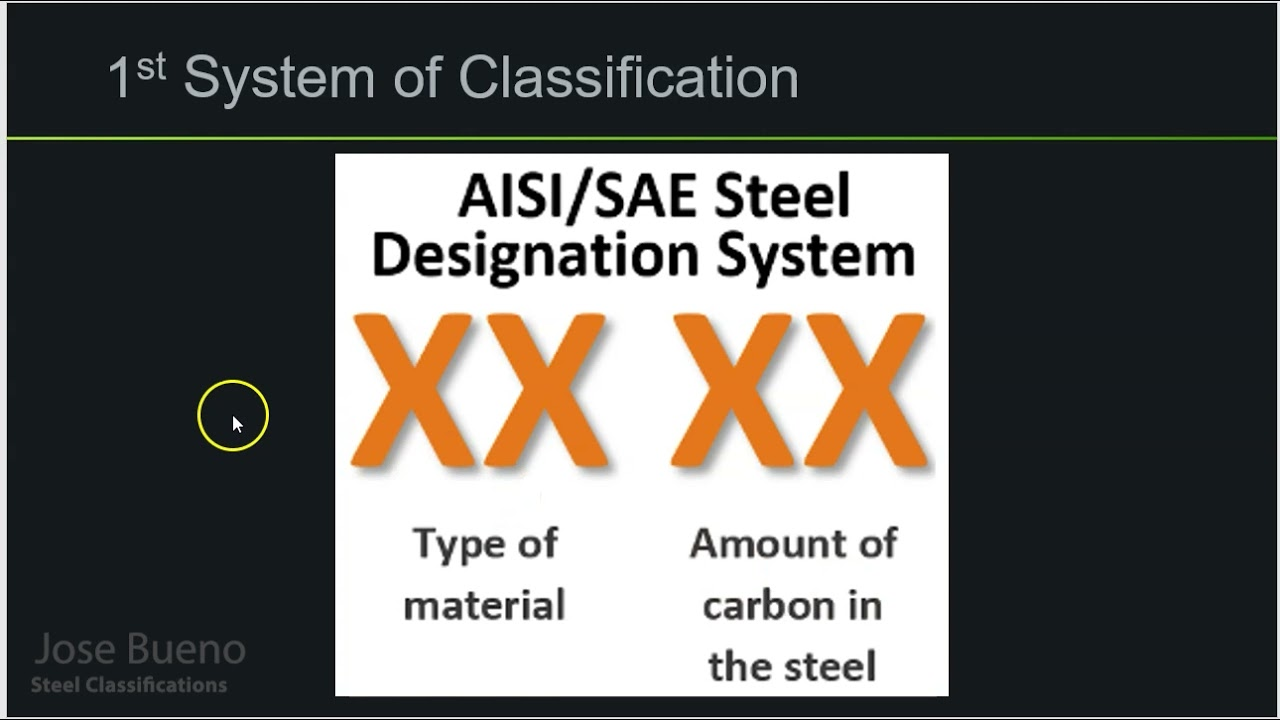
\includegraphics[height=6cm,width=1\textwidth,keepaspectratio]{identifying_steel_video.jpg}}
        \label{fig:identifying_steel_video.jpg}
    \end{figure}
\end{frame}



% \begin{frame}[t]{Reference material}
%     \framesubtitle{}
%     \begin{enumerate}
%         \item \href{https://youtu.be/PaGJwOPg2kU}{Understanding steels (eng)}
%         \item \href{https://youtu.be/WSRqJdT2COE}{Understanding Material Strength, Ductility and Toughness (eng)}
%         \item \href{https://disk.yandex.ru/i/pmZGYsEMQlrWTA}{Musa 1st lecture}
%         \item \href{https://disk.yandex.ru/i/RtD8vtzjY-XxyQ}{Musa 2nd lecture}
%     \end{enumerate}

%     % 
% \end{frame}



\fbckg{fibeamer/figs/last_page.png}
\frame[plain]{}

\end{document}
